\documentclass[a0,portrait]{a0poster}

\usepackage{multicol}
\columnsep=100pt
\columnseprule=3pt

\usepackage[svgnames]{xcolor}

\usepackage{times}
\usepackage{palatino}
\usepackage[none]{hyphenat}
\usepackage{graphicx}
\graphicspath{{figures/}}
\usepackage{booktabs}
\usepackage[font=small,labelfont=bf]{caption}
\usepackage{amsfonts, amsmath, amsthm, amssymb}
\usepackage{wrapfig}
\usepackage{lipsum,adjustbox}
\usepackage[absolute,overlay]{textpos}
\usepackage{multirow}
\usepackage{titlesec}
\usepackage[inline]{enumitem}
\usepackage{url}
\usepackage{tikz,pgfplots,pgfplotstable}
\usepackage{tikz-dependency}
\usetikzlibrary{arrows.meta}
\captionsetup{labelformat=empty}

\begin{document}

\begin{center}
	\veryHuge \color{NavyBlue} \textbf{Universal Dependency Parsing \\
	with a General Transition-Based DAG Parser}
\end{center}
\begin{minipage}[b]{0.57\linewidth}
\LARGE \textbf{Daniel Hershcovich}\textsuperscript{1,2} \&
	   \textbf{Omri Abend}\textsuperscript{2} \&
	   \textbf{Ari Rappoport}\textsuperscript{2} \\[0.5cm]
\large $^1$The Edmond and Lily Safra Center for Brain Sciences \\
  $^2$School of Computer Science and Engineering
  \setlength{\columnseprule}{0pt}
  \setlength\multicolsep{-20pt}
  \begin{multicols}{2}
  The Hebrew University of Jerusalem \\
  \texttt{\{danielh,oabend,arir\}@cs.huji.ac.il}
  \end{multicols}
\end{minipage}
\hfill
\begin{minipage}[b]{.1\linewidth}

\includegraphics[width=\linewidth]{elsc_logo.png}
\end{minipage}
\begin{minipage}[b]{.18\linewidth}

\includegraphics[width=\linewidth]{huji_banner.png}

\includegraphics[width=1.04\linewidth]{cse_banner.jpg}
\end{minipage}
\begin{minipage}[b]{.07\linewidth}

\includegraphics[width=\linewidth]{huji_logo.jpg}
\end{minipage}

\vspace{1cm}
\titlespacing*{\section}{0pt}{8mm}{5mm}

%----------------------------------------------------------------------------------------


\begin{adjustbox}{margin=5mm,frame,minipage=.51\linewidth,center}
\Large\color{Navy}
We present a \textbf{general DAG parser} for UCCA, AMR, SDP and UD,
and show that \textbf{multitask learning} improves UCCA parsing.
\end{adjustbox}


\begin{multicols}{2}


\color{Black}

Training data for parsing semantic representations is scarce.
We consider four schemes:
\begin{itemize}[labelsep=1em]
{\color{Indigo} \item[\textbf{UCCA}:] Intuitive, cross-lingual, and modular semantic representation.
    \textit{Primary edges} form a tree. \textit{Remote edges} (dashed) allow reentrancy,
    creating a directed acyclic graph \cite{abend2013universal}.}
{\color{DarkGreen} \item[\textbf{AMR}:] Abstract graph on concepts and constants.
    Rooted DAG with labeled nodes and edges.
    Encodes named entities, argument structure, semantic roles, word sense, coreference \cite{banarescu2013abstract}.}
{\color{DarkRed} \item[\textbf{SDP}:] Set of related bilexical semantic DAG schemes: DM, PAS, PSD and CCD.
    We use \textbf{DM}~(DELPH-IN~MRS).
    Encodes argument structure for many predicate types \cite{oepen2016towards}.}
{\color{DarkBlue} \item[\textbf{UD}:] Cross-lingual syntactic bilexical tree.
    Encodes syntactic relations between words \cite{nivre2016universal}. \\
    \textbf{UD$^{++}$} (Enhanced++ UD) adds and augments edges, creating a bilexical DAG
    \cite{SCHUSTER16.779}.}
\end{itemize}

\begin{minipage}{.8\columnwidth}
  \color{Indigo}
  \begin{center}
    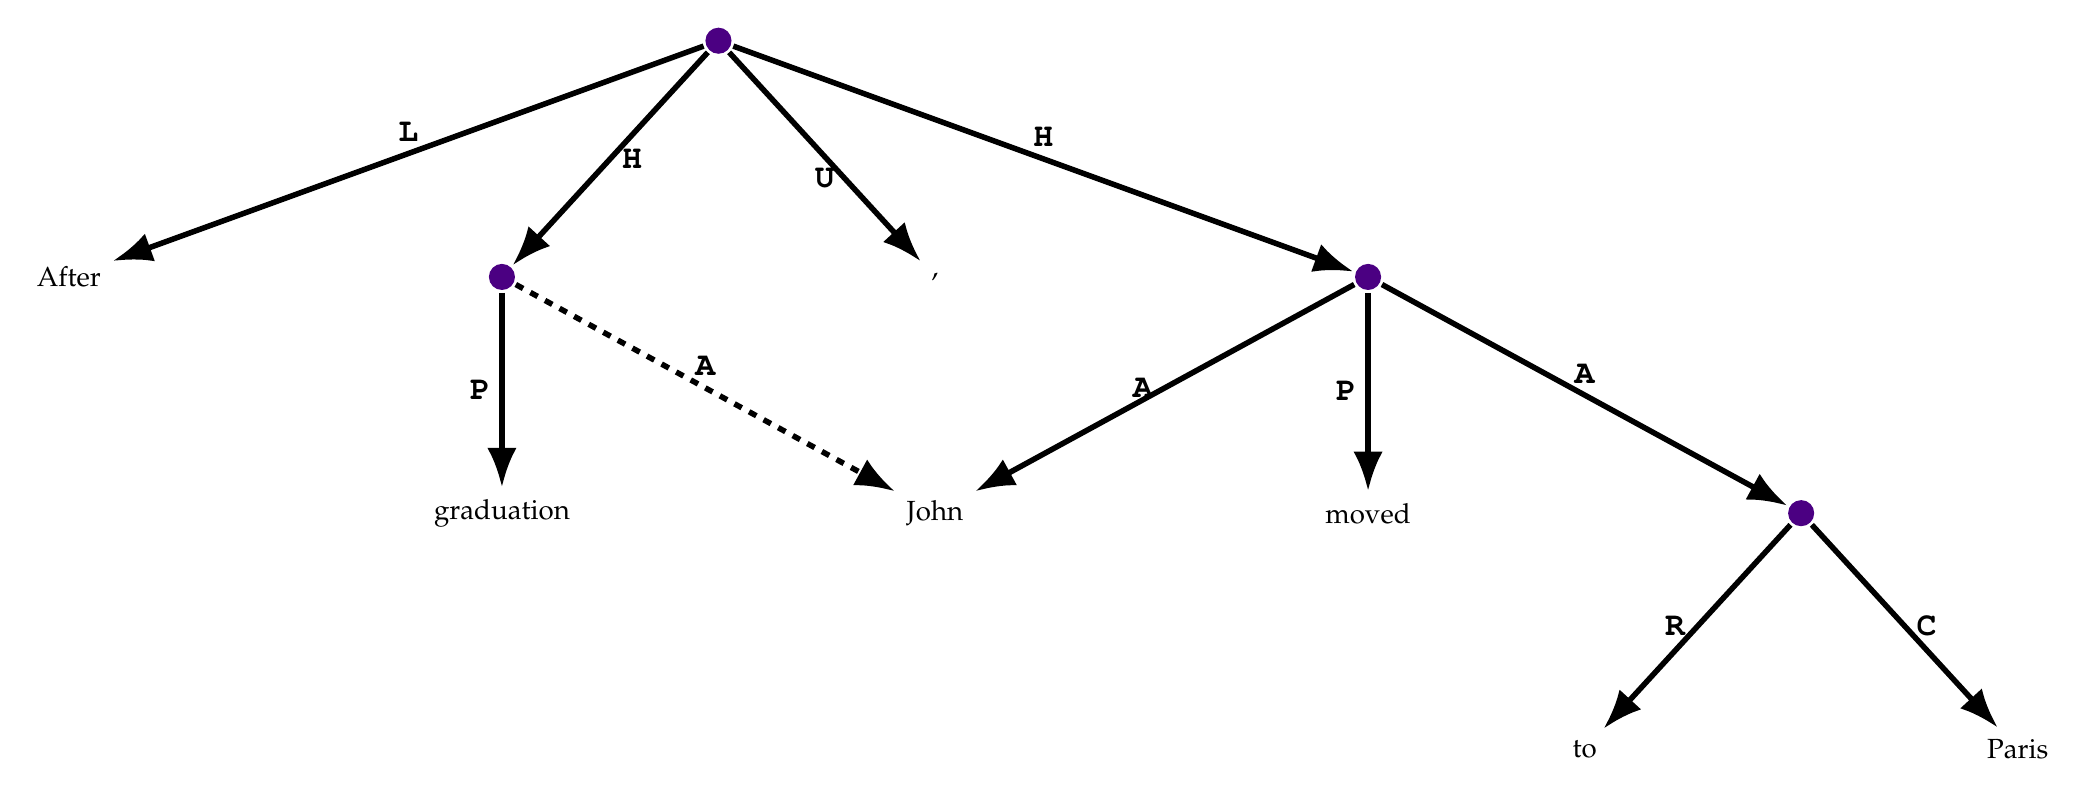
\begin{tikzpicture}[level distance=3cm, sibling distance=55mm, -{Latex[length=5mm]}, line width=2pt,
        every node/.append style={font=\large\bf\ttfamily},
        every circle node/.append style={fill=Indigo}]
      \tikzstyle{word} = [font=\rmfamily,color=black]
      \node (ROOT) [circle] {}
        child {node (After) [word] {After} edge from parent node[above] {L}}
        child {node (graduation) [circle] {}
        {
          child {node [word] {graduation} edge from parent node[left] {P}}
        } edge from parent node[right] {H} }
        child {node [word] {,} edge from parent node[below] {U}}
        child {node (moved) [circle] {}
        {
          child {node (John) [word] {John} edge from parent node[left] {A}}
          child {node [word] {moved} edge from parent node[left] {P}}
          child {node [circle] {}
          {
            child {node [word] {to} edge from parent node[left] {R}}
            child {node [word] {Paris} edge from parent node[right] {C}}
          } edge from parent node[above] {A} }
        } edge from parent node[above] {H} }
        ;
      \draw[dashed,-{Latex[length=5mm]}] (graduation) to node [above] {A} (John);
    \end{tikzpicture}
  \captionof{figure}{\color{Indigo} Universal Conceptual Cognitive Annotation (UCCA).}
  \end{center}
\end{minipage}
\hfill
\begin{minipage}{.2\columnwidth}
  \begin{center}
  \begin{adjustbox}{margin=2mm,frame,scale=.75}
  \color{Indigo}
  \begin{tabular}{>{\bf\ttfamily}cl}
	  P & process \\
	  S & state \\
	  A & participant \\
	  L & linker \\
	  H & linked scene \\
	  C & center \\
	  E & elaborator \\
	  D & adverbial \\
	  R & relator \\
	  N & connector \\
	  U & punctuation \\
	  F & function unit \\
	  G & ground
  \end{tabular}
  \end{adjustbox}
  \captionof{table}{\color{Indigo} UCCA edge labels.}
  \end{center}
\end{minipage}

\hspace{-35mm}
\begin{minipage}{.50\columnwidth}
  \begin{center}
  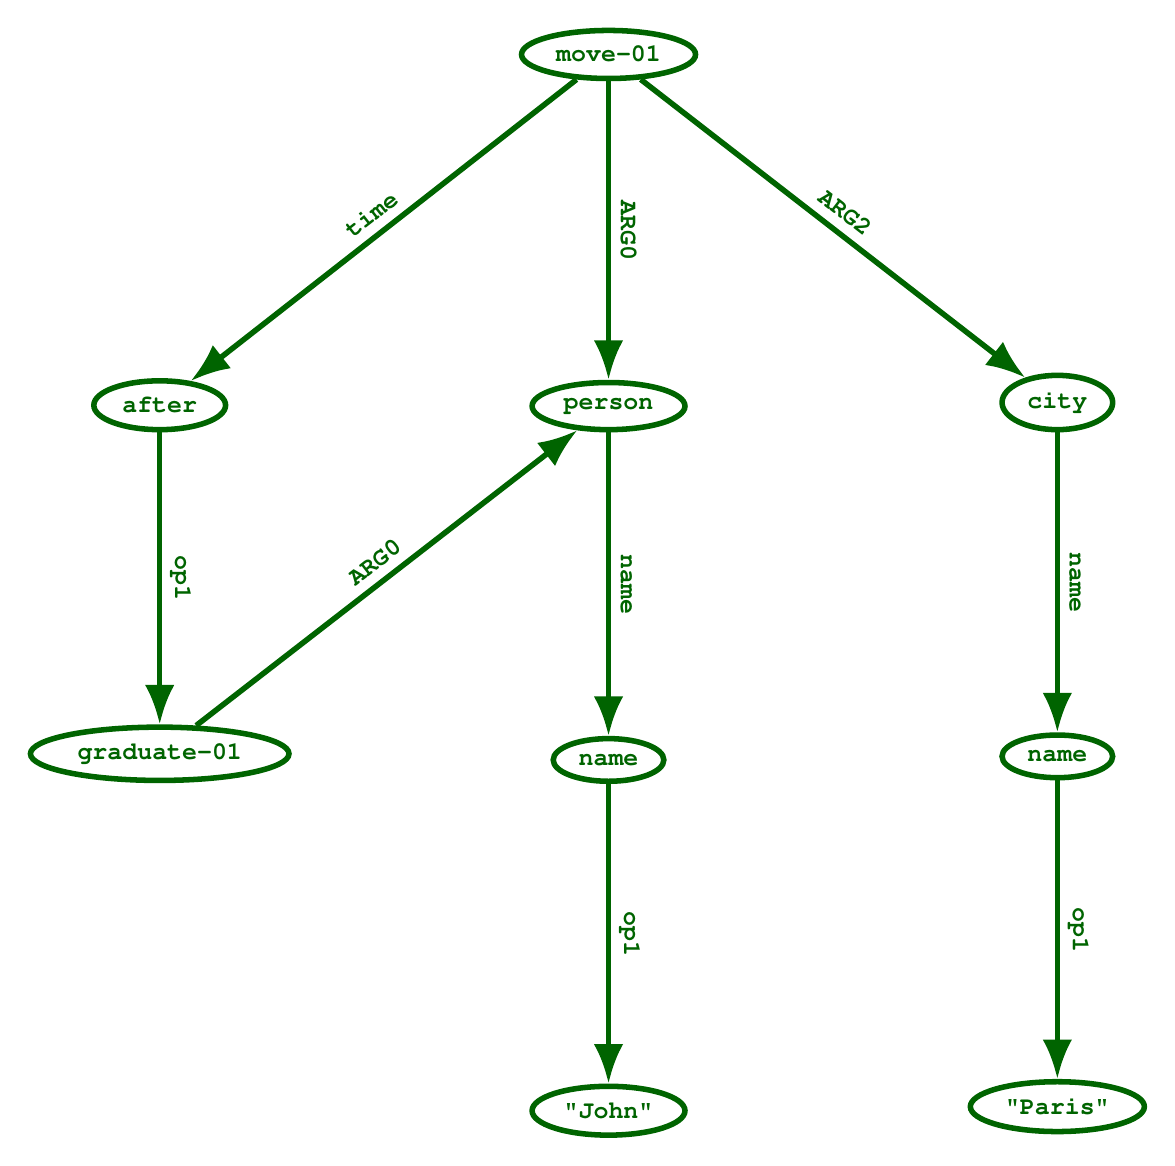
\begin{tikzpicture}[-{Latex[length=5mm]}, color=DarkGreen, level distance=48mm, line width=2pt,
      every node/.append style={sloped,anchor=south,auto=false,font=\small\bf\ttfamily},
      level 1/.style={sibling distance=57mm}]
    \node (ROOT) [draw=DarkGreen,ellipse] {move-01}
      child {node [draw=DarkGreen,ellipse] {after}
      {
            child {node (graduation) [draw=DarkGreen,ellipse] {graduate-01} edge from parent node {op1} }
      } edge from parent node {time} }
      child {node (John) [draw=DarkGreen,ellipse] {person}
      {
        child {node [draw=DarkGreen,ellipse] {name}
        {
            child {node [draw=DarkGreen,ellipse] {"John"} edge from parent node {op1} }
        } edge from parent node {name} }
      } edge from parent node {ARG0} }
      child {node [draw=DarkGreen,ellipse] {city}
      {
        child {node [draw=DarkGreen,ellipse] {name}
        {
            child {node [draw=DarkGreen,ellipse] {"Paris"} edge from parent node {op1} }
        } edge from parent node {name} }
      } edge from parent node {ARG2} }
      ;
      \draw (graduation) to node {ARG0} (John);
  \end{tikzpicture}
  \captionof{figure}{\color{DarkGreen} Abstract Meaning Representation (AMR).}
  \end{center}
\end{minipage}
\begin{minipage}{.55\columnwidth}
    \begin{center}
    \begin{dependency}[edge style={-{Latex[length=4mm]}, color=DarkRed, line width=2pt},
        text only label, label style={above, color=DarkRed, font=\bf\ttfamily}, font=\small]
    \begin{deptext}[column sep=.8em,ampersand replacement=\^, color=DarkRed]
    After \^ graduation \^ , \^ John \^ moved \^ to \^ Paris \\
    \end{deptext}
        \depedge[edge unit distance=1em]{1}{2}{ARG2}
        \depedge[edge unit distance=1em, edge start x offset=-4mm]{5}{4}{ARG1}
        \depedge[edge unit distance=1em, edge end x offset=-3mm]{1}{5}{ARG1}
        \deproot[edge unit distance=1.25em]{5}{top}
        \depedge[edge unit distance=2em, edge start x offset=1mm, edge end x offset=3mm]{5}{7}{ARG2}
        \depedge[edge unit distance=1em, edge end x offset=5mm]{6}{5}{ARG1}
        \depedge[edge unit distance=1em]{6}{7}{ARG2}
    \end{dependency}
    \captionof{figure}{\color{DarkRed} Semantic Dependency Parsing (SDP): DM representation.}
    \vspace{7mm}
    \begin{dependency}[edge style={-{Latex[length=4mm]}, color=DarkBlue, line width=2pt},
        text only label, label style={above, color=DarkBlue, font=\bf\ttfamily}, font=\small]
    \begin{deptext}[column sep=.8em,ampersand replacement=\^, color=DarkBlue]
    After \^ graduation \^ , \^ John \^ moved \^ to \^ Paris \\
    \end{deptext}
        \depedge[edge unit distance=1em]{2}{1}{case}
        \depedge[edge unit distance=1em]{4}{3}{punct}
        \depedge[edge unit distance=1em, edge start x offset=-4mm]{5}{4}{nsubj}
        \depedge[edge unit distance=1em, edge end x offset=-3mm]{2}{5}{obl}
        \depedge[edge unit distance=1em]{7}{6}{case}
        \deproot[edge unit distance=1em]{5}{root}
        \depedge[edge unit distance=1.5em, edge start x offset=1mm]{5}{7}{obl}
    \end{dependency}
  \captionof{figure}{\color{DarkBlue} Universal Dependencies (UD).}
  \end{center}
\end{minipage}

\vspace{5mm}

Semantic representations
share much of their content \cite{abend2017state}.

\textbf{Multitask learning} exploits task overlap,
effectively extending the training data.

We focus on UCCA parsing due to its small training set.

As auxiliary tasks, we use \textbf{unlabeled}
{\color{DarkGreen} AMR}, {\color{DarkRed} SDP} and {\color{DarkBlue} UD} parsing.

\hrule

\section*{Data}

\begin{itemize*}
\item [\textbf{\color{Indigo} UCCA}:] \color{Indigo} (1) English Wikipedia (\textbf{Wiki});
(2) \textit{Twenty Thousand Leagues Under the Sea} (\textbf{20K}),
annotated in English (small, only test) French (small), and German
(pre-release, noisy).
\item [\{\textbf{\color{DarkGreen} AMR}:] \color{DarkGreen} LDC2017T10 (English).
\item [\textbf{\color{DarkRed} SDP}:] \color{DarkRed} DM part from SDP 2016 (English).
\item [\textbf{\color{DarkBlue} UD}:] {\color{DarkBlue} v2.1 treebanks:
English (UD$^{++}$), French and German.}\}:
\end{itemize*}
Only for training.
\hfill Number of sentences per dataset:

\hspace{-35mm}
\begin{minipage}{.4\columnwidth}
\pgfplotstableread[row sep=\\,col sep=&]{
	corpus & total & train & dev & test \\
	\color{DarkBlue} \textbf{UD} & 17062 & 9062 & 0 & 0 \\
	\color{DarkRed} \textbf{SDP} & 33964 & 10964 & 0 & 0 \\
	\color{DarkGreen} \textbf{AMR} & 36521 & 11521 & 0 & 0 \\
	\color{Indigo} \textbf{Wiki} & 5225 & 4268 & 454 & 503 \\
	\color{Indigo} \textbf{20K} & 506 & 0 & 0 & 506 \\
    }\english
\begin{center}
    \begin{tikzpicture}
    \begin{axis}[
    xbar stacked,
    width=13cm,
    height=9cm,
    xmin=0,
    xmax=15000,
    xtick=\empty,
    ytick=data,
    yticklabels from table={\english}{corpus}
    ]
    \draw[black] decorate [decoration={zigzag}] {(axis cs:8600,-4) -- (axis cs:8600,5)};
    \addplot [fill=green!80] table [x=train,meta=corpus,y expr=\coordindex] {\english};
    \addplot [fill=blue!60] table [x=dev,y expr=\coordindex] {\english};
    \addplot [fill=red!60, point meta=explicit symbolic,nodes near coords, nodes near coords align={anchor=west}] table [x=test,y expr=\coordindex,meta=total] {\english};
    \end{axis}
    \end{tikzpicture}
    \captionof{figure}{\hspace{35mm} \textbf{English} corpora.}
\end{center}
\end{minipage}
\hspace{1mm}
\begin{minipage}{.34\columnwidth}
\pgfplotstableread[row sep=\\,col sep=&]{
	corpus & total & train & dev & test \\
	UD & 32347 & 11347 & 0 & 0 \\
	UCCA 20K & 547 & 413 & 67 & 67 \\
    }\french
\begin{center}
    \begin{tikzpicture}
    \begin{axis}[
    xbar stacked,
    width=13cm,
    height=9cm,
    xmin=0,
    xmax=15000,
    xtick=\empty,
    ytick=\empty,
    yticklabels=\empty
    ]
    \draw[black] decorate [decoration={zigzag}] {(axis cs:8600,-4) -- (axis cs:8600,5)};
    \addplot [fill=green!80] table [x=train,y expr=\coordindex] {\french};
    \addplot [fill=blue!60] table [x=dev,y expr=\coordindex] {\french};
    \addplot [fill=red!60, point meta=explicit symbolic, nodes near coords, nodes near coords align={anchor=west}] table [x=test,y expr=\coordindex,meta=total] {\french};
    \end{axis}
    \end{tikzpicture}
    \captionof{figure}{\textbf{French} corpora.}
\end{center}
\end{minipage}
\begin{minipage}{.34\columnwidth}
\pgfplotstableread[row sep=\\,col sep=&]{
	corpus & total & train & dev & test \\
	UD & 13814 & 9814 & 0 & 0 \\
	UCCA 20K & 6154 & 3429 & 561 & 2164 \\
    }\german
\begin{center}
    \begin{tikzpicture}
    \begin{axis}[
    xbar stacked,
    width=13cm,
    height=9cm,
    xmin=0,
    xmax=15000,
    xtick=\empty,
    ytick=\empty,
    legend style={at={(axis cs:10000,.8)},anchor=north west},
    yticklabels=\empty
    ]
    \draw[black] decorate [decoration={zigzag}] {(axis cs:9200,-4) -- (axis cs:9200,5)};
    \addplot [fill=green!80] table [x=train,y expr=\coordindex] {\german};
    \addplot [fill=blue!60] table [x=dev,y expr=\coordindex] {\german};
    \addplot [fill=red!60, point meta=explicit symbolic, nodes near coords, nodes near coords align={anchor=west}] table [x=test, meta=corpus,y expr=\coordindex,meta=total] {\german};
    \legend{train,dev,test}
    \end{axis}
    \end{tikzpicture}
    \captionof{figure}{\textbf{German} corpora.}
\end{center}
\end{minipage}

\vspace{5mm}

Domains differ, too:
\begin{center}
	\begin{tabular}{llll}
		\color{Indigo} \textbf{UCCA}  & \color{DarkGreen} \textbf{AMR}  & \color{DarkRed} \textbf{SDP}  & \color{NavyBlue} \textbf{UD}  \\
		Wikipedia & blogs & news & blogs \\ books & news && news \\ & emails && emails \\ & reviews && reviews \\ &&& Q\&A
	\end{tabular}
\end{center}

\hrule


\section*{TUPA: A Transition-Based DAG Parser}

We extend TUPA, a general DAG parser,
which has been proposed as a UCCA parser \cite{hershcovich2017a}. \\
It is a transition-based parser supporting reentrancy, discontinuity and non-terminal nodes.

\scalebox{.9}{
\begin{minipage}{.55\columnwidth}
	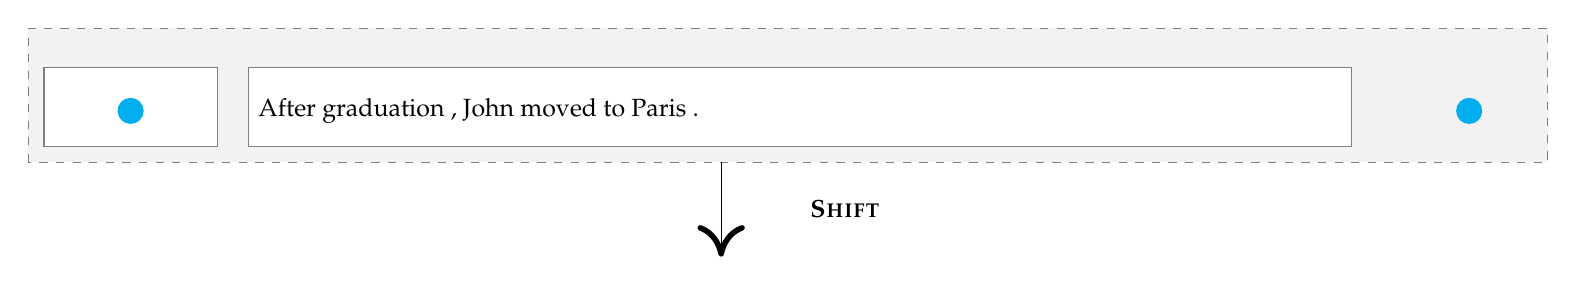
\begin{tikzpicture}[level distance=15mm, sibling distance=4cm, font=\small]
	\draw[color=gray,dashed,fill=lightgray!20] (.2,-.2) rectangle (19.5,1.5);
	\draw[color=gray,fill=white] (.4,0) rectangle (2.6,1);
	\node[fill=cyan, circle] at (1.5,.45) {};
	\draw[color=gray,fill=white] (3,0) rectangle (17,1);
	\node[anchor=west] at (3,.45) {After graduation , John moved to Paris .};
	\node[fill=cyan, circle] at (18.5,.45) {};
	\node[anchor=west] at (10,-.8) {\bf\small\textsc{Shift}};
	\draw[arrows={->[line width=2pt,length=4mm,width=6mm]}] (9,-.2) -- (9,-1.4);
	\end{tikzpicture}
	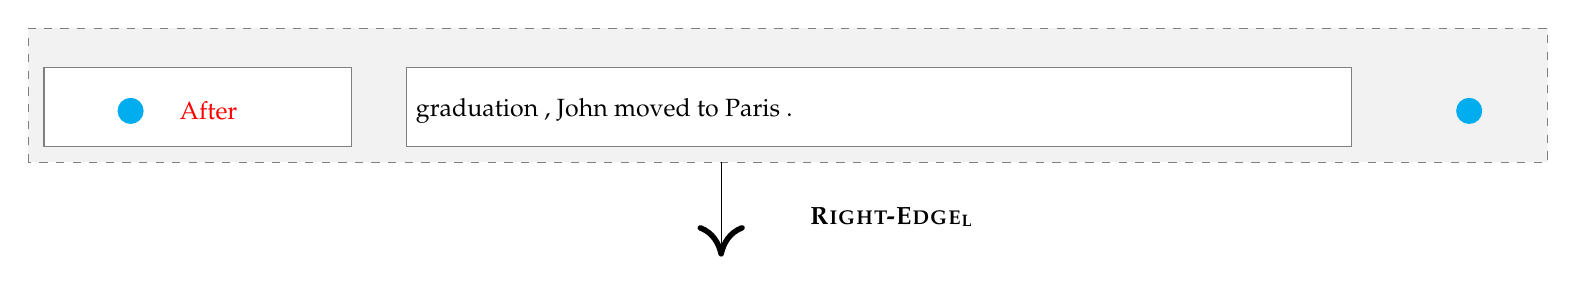
\begin{tikzpicture}[level distance=15mm, sibling distance=4cm, font=\small]
	\draw[color=gray,dashed,fill=lightgray!20] (.2,-.2) rectangle (19.5,1.5);
	\draw[color=gray,fill=white] (.4,0) rectangle (4.3,1);
	\node[fill=cyan, circle] at (1.5,.45) {};
	\node[color=red,anchor=west] at (2,.45) {After};
	\draw[color=gray,fill=white] (5,0) rectangle (17,1);
	\node[anchor=west] at (5,.45) {graduation , John moved to Paris .};
	\node[fill=cyan, circle] at (18.5,.45) {};
	\node[anchor=west] at (10,-.9) {\bf\small\textsc{Right-Edge\textsubscript L}};
	\draw[arrows={->[line width=2pt,length=4mm,width=6mm]}] (9,-.2) -- (9,-1.4);
	\end{tikzpicture}
	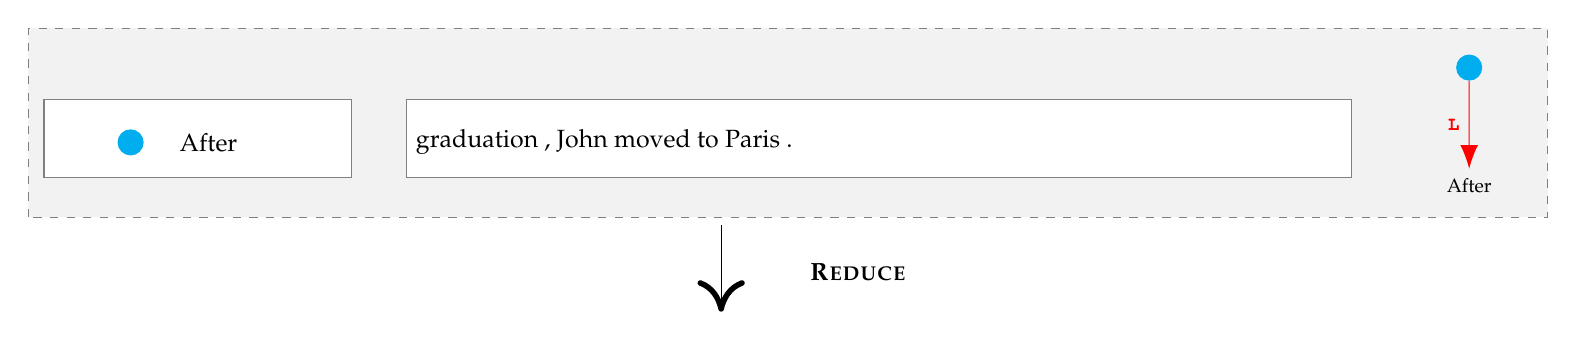
\begin{tikzpicture}[level distance=15mm, sibling distance=4cm, font=\small, -{Latex[length=3mm]}]
	\draw[color=gray,dashed,fill=lightgray!20] (.2,-.5) rectangle (19.5,1.9);
	\draw[color=gray,fill=white] (.4,0) rectangle (4.3,1);
	\node[fill=cyan, circle] at (1.5,.45) {};
	\node[anchor=west] at (2,.45) {After};
	\draw[color=gray,fill=white] (5,0) rectangle (17,1);
	\node[anchor=west] at (5,.45) {graduation , John moved to Paris .};
	\node[fill=cyan, circle] at (18.5,1.4) {}
	  child {node[font=\scriptsize] {After} edge from parent [red] node[font=\scriptsize\bf\ttfamily,left] {L}};
	\node[anchor=west] at (10,-1.2) {\bf\small\textsc{Reduce}};
	\draw[arrows={->[line width=2pt,length=4mm,width=6mm]}] (9,-.6) -- (9,-1.7);
	\end{tikzpicture}
	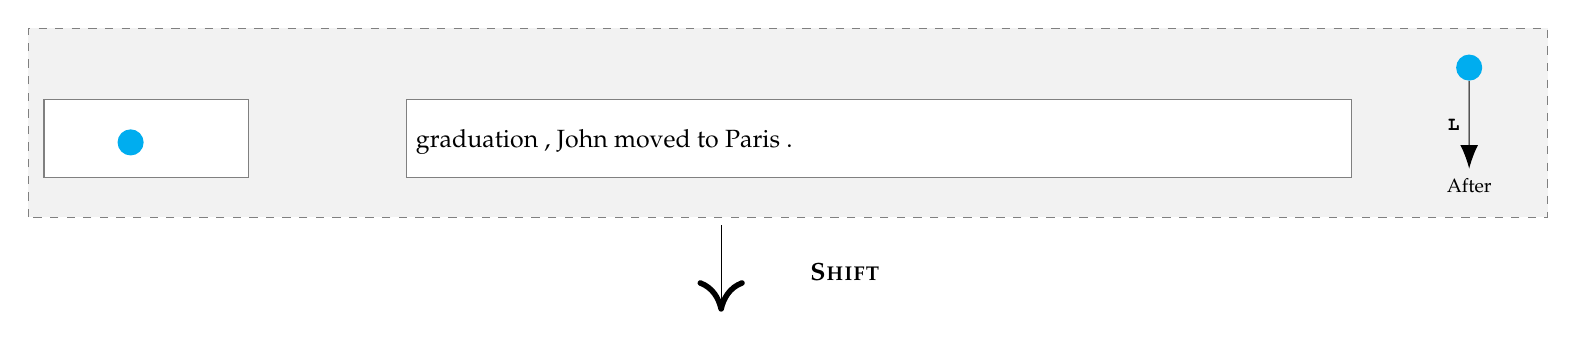
\begin{tikzpicture}[level distance=15mm, sibling distance=4cm, font=\small, -{Latex[length=3mm]}]
	\draw[color=gray,dashed,fill=lightgray!20] (.2,-.5) rectangle (19.5,1.9);
	\draw[color=gray,fill=white] (.4,0) rectangle (3,1);
	\node[fill=cyan, circle] at (1.5,.45) {};
	\draw[color=gray,fill=white] (5,0) rectangle (17,1);
	\node[anchor=west] at (5,.45) {graduation , John moved to Paris .};
	\node[fill=cyan, circle] at (18.5,1.4) {}
	  child {node[font=\scriptsize] {After} edge from parent node[font=\scriptsize\bf\ttfamily,left] {L}};
	\node[anchor=west] at (10,-1.2) {\bf\small\textsc{Shift}};
	\draw[arrows={->[line width=2pt,length=4mm,width=6mm]}] (9,-.6) -- (9,-1.7);
	\end{tikzpicture}
	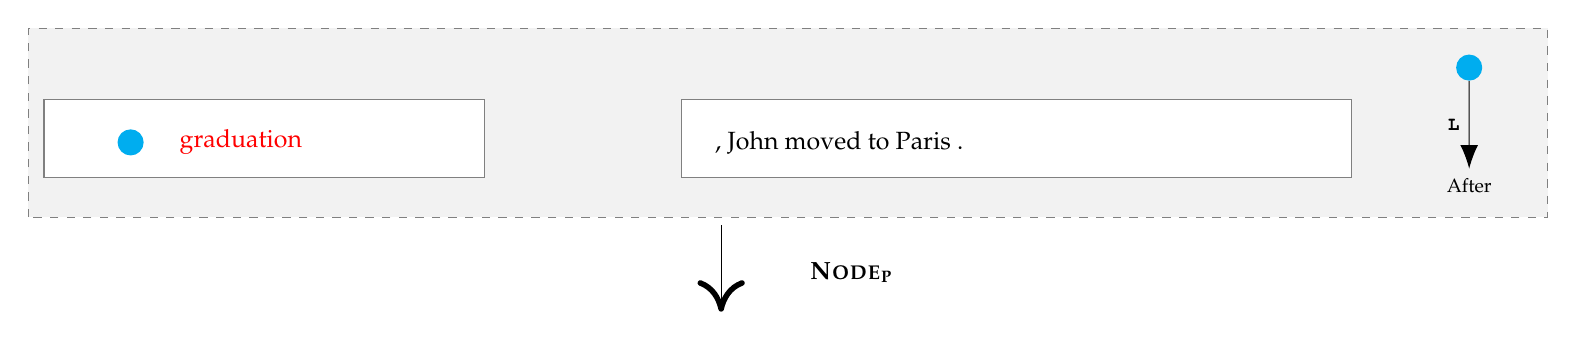
\begin{tikzpicture}[level distance=15mm, sibling distance=4cm, font=\small, -{Latex[length=3mm]}]
	\draw[color=gray,dashed,fill=lightgray!20] (.2,-.5) rectangle (19.5,1.9);
	\draw[color=gray,fill=white] (.4,0) rectangle (6,1);
	\node[fill=cyan, circle] at (1.5,.45) {};
	\node[color=red,anchor=west] at (2,.45) {graduation};
	\draw[color=gray,fill=white] (8.5,0) rectangle (17,1);
	\node[anchor=west] at (8.8,.45) {, John moved to Paris .};
	\node[fill=cyan, circle] at (18.5,1.4) {}
	  child {node[font=\scriptsize] {After} edge from parent node[font=\scriptsize\bf\ttfamily,left] {L}};
	\node[anchor=west] at (10,-1.2) {\bf\small\textsc{Node\textsubscript P}};
	\draw[arrows={->[line width=2pt,length=4mm,width=6mm]}] (9,-.6) -- (9,-1.7);
	\end{tikzpicture}
	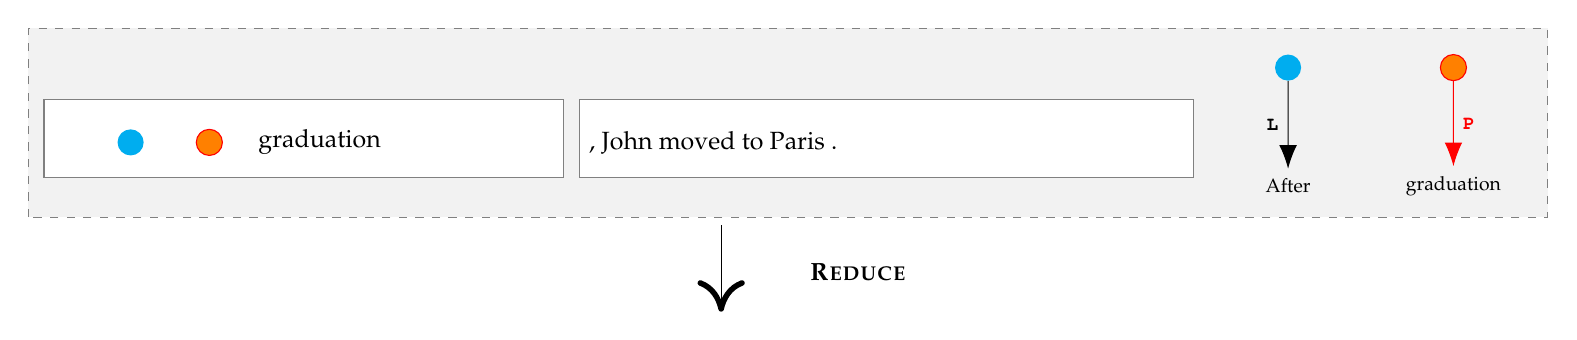
\begin{tikzpicture}[level distance=15mm, sibling distance=4cm, font=\small, -{Latex[length=3mm]}]
	\draw[color=gray,dashed,fill=lightgray!20] (.2,-.5) rectangle (19.5,1.9);
	\draw[color=gray,fill=white] (.4,0) rectangle (7,1);
	\node[fill=cyan, circle] at (1.5,.45) {};
	\node[fill=orange, draw=red, circle] at (2.5,.45) {};
	\node[anchor=west] at (3,.45) {graduation};
	\draw[color=gray,fill=white] (7.2,0) rectangle (15,1);
	\node[anchor=west] at (7.2,.45) {, John moved to Paris .};
	\node[fill=cyan, circle] at (16.2,1.4) {}
	  child {node[font=\scriptsize] {After} edge from parent node[font=\scriptsize\bf\ttfamily,left] {L}};
	\node[fill=orange, draw=red, circle] at (18.3,1.4) {}
	  child {node[font=\scriptsize] {graduation} edge from parent [red] node[font=\scriptsize\bf\ttfamily,right] {P}};
	\node[anchor=west] at (10,-1.2) {\bf\small\textsc{Reduce}};
	\draw[arrows={->[line width=2pt,length=4mm,width=6mm]}] (9,-.6) -- (9,-1.7);
	\end{tikzpicture}
\end{minipage}
\hspace{1cm}
\begin{minipage}{.4\columnwidth}
	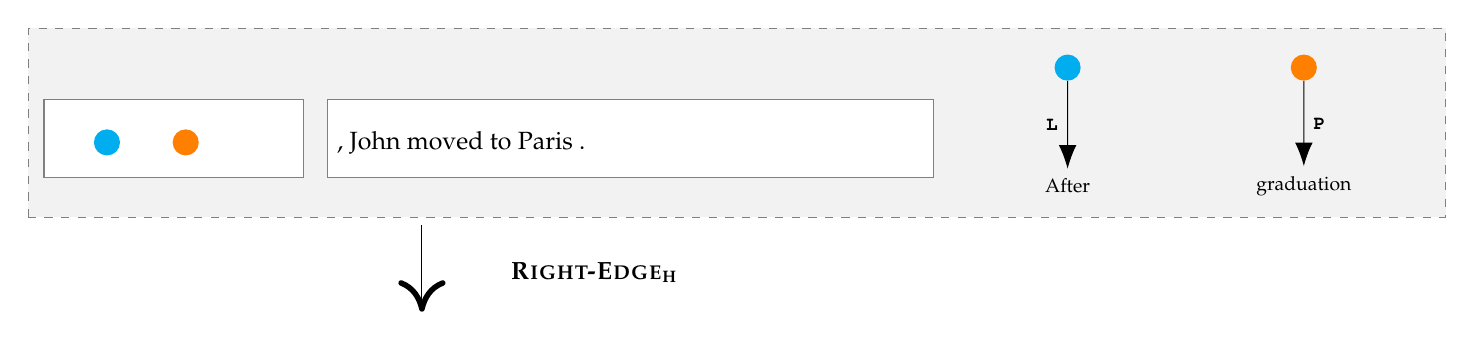
\begin{tikzpicture}[level distance=15mm, sibling distance=4cm, font=\small, -{Latex[length=3mm]}]
	\draw[color=gray,dashed,fill=lightgray!20] (0,-.5) rectangle (18,1.9);
	\draw[color=gray,fill=white] (0.2,0) rectangle (3.5,1);
	\node[fill=cyan, circle] at (1,.45) {};
	\node[fill=orange, circle] at (2,.45) {};
	\draw[color=gray,fill=white] (3.8,0) rectangle (11.5,1);
	\node[anchor=west] at (3.8,.45) {, John moved to Paris .};
	\node[fill=cyan, circle] at (13.2,1.4) {}
	  child {node[font=\scriptsize] {After} edge from parent node[font=\scriptsize\bf\ttfamily,left] {L}};
	\node[fill=orange, circle] at (16.2,1.4) {}
	  child {node[font=\scriptsize] {graduation} edge from parent node[font=\scriptsize\bf\ttfamily,right] {P}};
	\node[anchor=west] at (6,-1.2) {\bf\small\textsc{Right-Edge\textsubscript H}};
	\draw[arrows={->[line width=2pt,length=4mm,width=6mm]}] (5,-.6) -- (5,-1.7);
	\end{tikzpicture}
	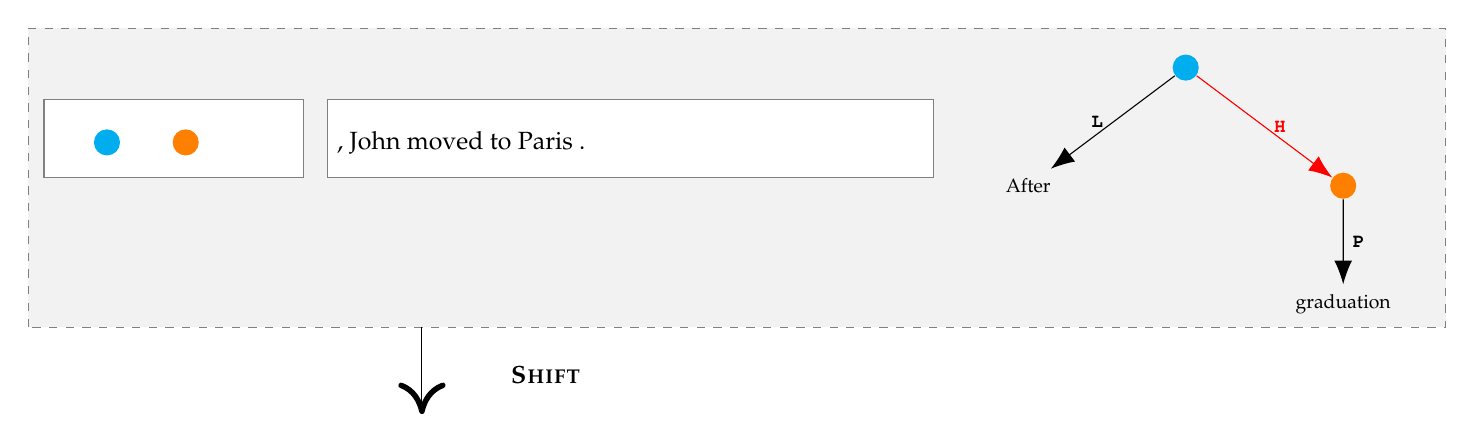
\begin{tikzpicture}[level distance=15mm, sibling distance=4cm, font=\small, -{Latex[length=3mm]}]
	\draw[color=gray,dashed,fill=lightgray!20] (0,-1.9) rectangle (18,1.9);
	\draw[color=gray,fill=white] (0.2,0) rectangle (3.5,1);
	\node[fill=cyan, circle] at (1,.45) {};
	\node[fill=orange, circle] at (2,.45) {};
	\draw[color=gray,fill=white] (3.8,0) rectangle (11.5,1);
	\node[anchor=west] at (3.8,.45) {, John moved to Paris .};
	\node[fill=cyan, circle] at (14.7,1.4) {}
	  child {node[font=\scriptsize] {After} edge from parent node[font=\scriptsize\bf\ttfamily,left] {L}}
	  child {node [fill=orange, circle] {}
	  {
	    child {node[font=\scriptsize] {graduation} edge from parent [black] node[font=\scriptsize\bf\ttfamily,right] {P}}
	  } edge from parent [red] node[font=\scriptsize\bf\ttfamily,right] {H} };
	\node[anchor=west] at (6,-2.5) {\bf\small\textsc{Shift}};
	\draw[arrows={->[line width=2pt,length=4mm,width=6mm]}] (5,-1.9) -- (5,-3);
	\end{tikzpicture}
	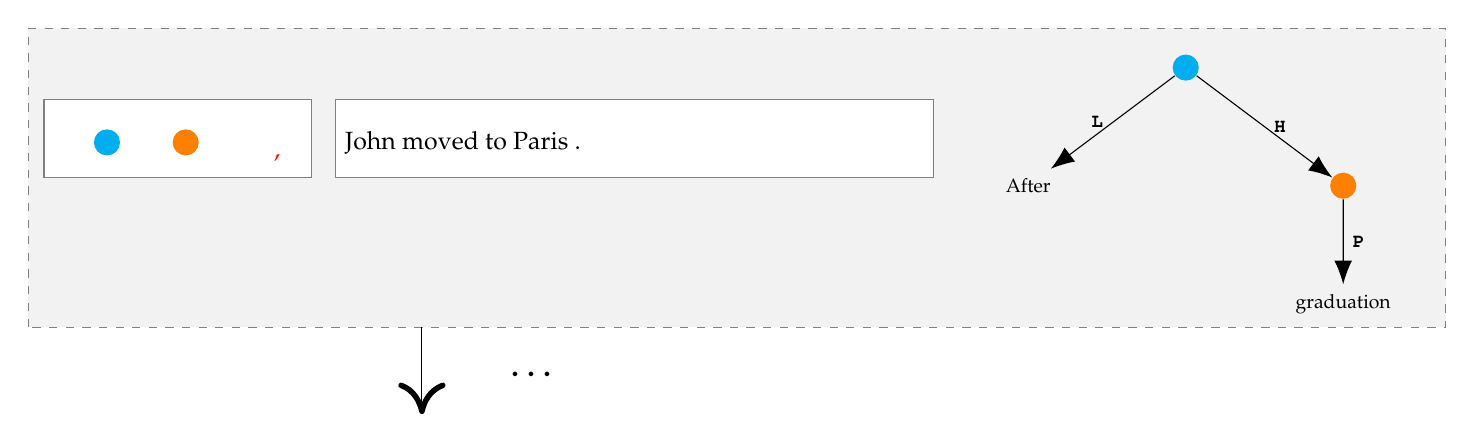
\begin{tikzpicture}[level distance=15mm, sibling distance=4cm, font=\small, -{Latex[length=3mm]}]
	\draw[color=gray,dashed,fill=lightgray!20] (0,-1.9) rectangle (18,1.9);
	\draw[color=gray,fill=white] (0.2,0) rectangle (3.6,1);
	\node[fill=cyan, circle] at (1,.45) {};
	\node[fill=orange, circle] at (2,.45) {};
	\node[color=red, anchor=west] at (3,.25) {,};
	\draw[color=gray,fill=white] (3.9,0) rectangle (11.5,1);
	\node[anchor=west] at (3.9,.45) {John moved to Paris .};
	\node[fill=cyan, circle] at (14.7,1.4) {}
	  child {node[font=\scriptsize] {After} edge from parent node[font=\scriptsize\bf\ttfamily,left] {L}}
	  child {node [fill=orange, circle] {}
	  {
	    child {node[font=\scriptsize] {graduation} edge from parent node[font=\scriptsize\bf\ttfamily,right] {P}}
	  } edge from parent node[font=\scriptsize\bf\ttfamily,right] {H} };
	\node[anchor=west] at (6,-2.5) {\Large \ldots};
	\draw[arrows={->[line width=2pt,length=4mm,width=6mm]}] (5,-1.9) -- (5,-3);
	\end{tikzpicture}
	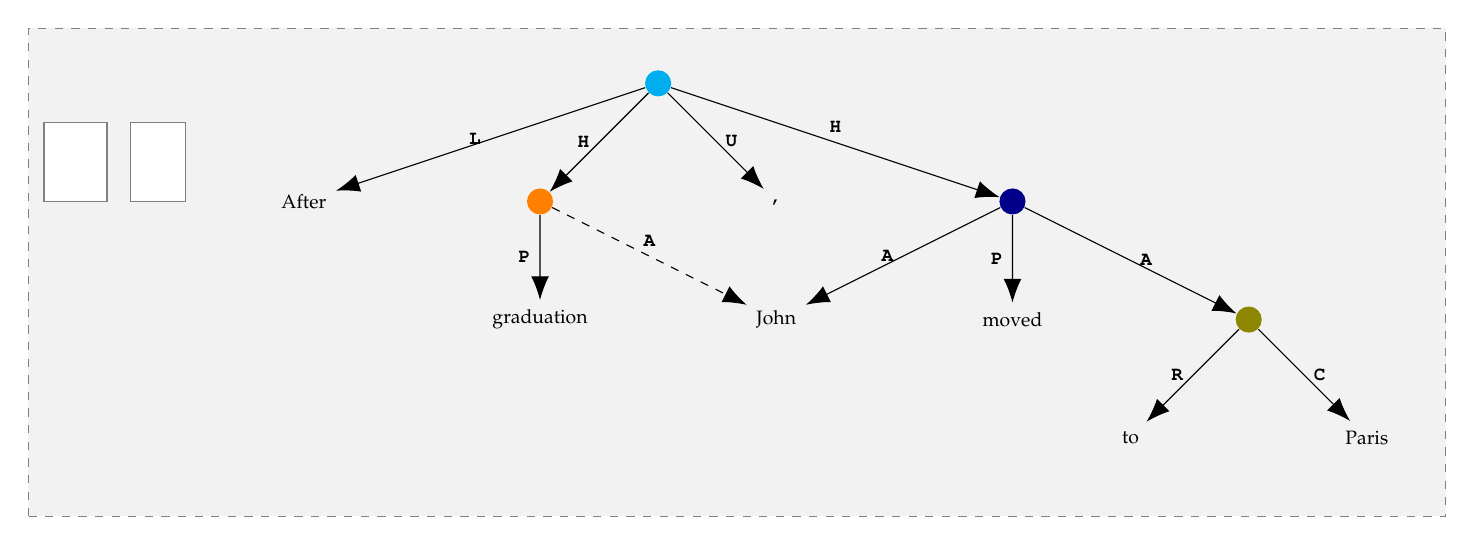
\begin{tikzpicture}[level distance=15mm, sibling distance=3cm, font=\small, -{Latex[length=3mm]}]
	\draw[color=gray,dashed,fill=lightgray!20] (0,-4) rectangle (18,2.2);
	\draw[color=gray,fill=white] (.2,0) rectangle (1,1);
	\draw[color=gray,fill=white] (1.3,0) rectangle (2,1);
    \node (ROOT) [fill=cyan,circle] at (8,1.5) {}
      child {node[font=\scriptsize] (After) {After} edge from parent node[font=\scriptsize\bf\ttfamily,left] {L}}
      child {node (graduation) [fill=orange,circle] {}
      {
        child {node[font=\scriptsize] {graduation} edge from parent node[font=\scriptsize\bf\ttfamily,left] {P}}
      } edge from parent node[font=\scriptsize\bf\ttfamily,left] {H} }
      child {node[font=\scriptsize\bf\ttfamily] {,} edge from parent node[font=\scriptsize\bf\ttfamily,right] {U}}
      child {node (moved) [fill=DarkBlue,circle] {}
      {
        child {node[font=\scriptsize] (John) {John} edge from parent node[font=\scriptsize\bf\ttfamily,left] {A}}
        child {node[font=\scriptsize] {moved} edge from parent node[font=\scriptsize\bf\ttfamily,left] {P}}
        child {node [fill=olive,circle] {}
        {
          child {node[font=\scriptsize] {to} edge from parent node[font=\scriptsize\bf\ttfamily,left] {R}}
          child {node[font=\scriptsize] {Paris} edge from parent node[font=\scriptsize\bf\ttfamily,right] {C}}
        } edge from parent node[font=\scriptsize\bf\ttfamily,right] {A} }
      } edge from parent node[font=\scriptsize\bf\ttfamily,above] {H} }
      ;
    \draw[dashed] (graduation) to node [font=\scriptsize\bf\ttfamily,above] {A} (John);
	\end{tikzpicture}
\end{minipage}
}

\vfill

\section*{Transition Classifier}

\begin{center}
   \vspace{-1mm}
   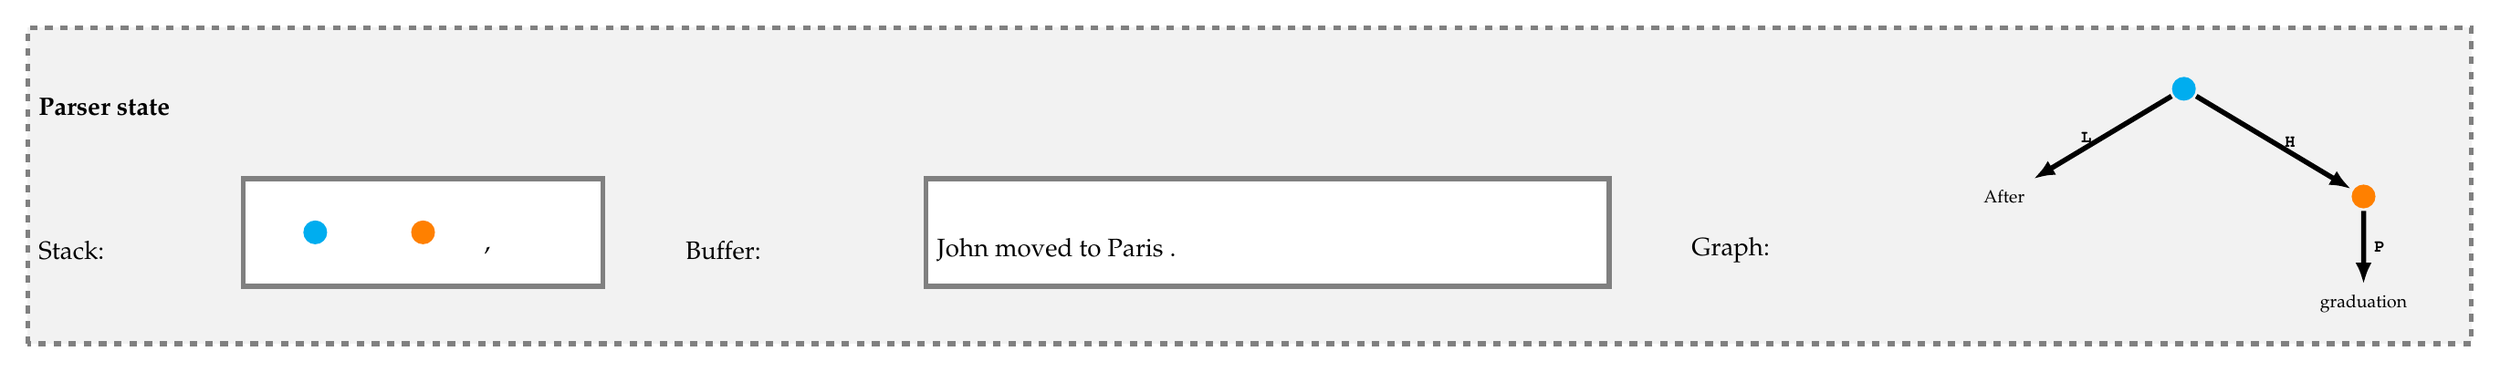
\begin{tikzpicture}[-{Latex[length=3mm]},level distance=15mm, sibling distance=5cm, line width=2pt]
   \draw[color=gray,dashed,fill=lightgray!20] (0,-.8) rectangle (34,3.6);
   \node[anchor=west] at (0,2.5) {\textbf{Parser state}};
   \node[anchor=west] at (0,.5) {Stack:};
   \draw[color=gray,fill=white] (3,0) rectangle (8,1.5);
   \node[fill=cyan, circle] at (4,.75) {};
   \node[fill=orange, circle] at (5.5,.75) {};
   \node[anchor=west] at (6.2,.5) {,};
   \node[anchor=west] at (9,.5) {Buffer:};
   \draw[color=gray,fill=white] (12.5,0) rectangle (22,1.5);
   \node[anchor=west] at (12.5,.5) {John moved to Paris .};
   \node[anchor=west] at (23,.5) {Graph:};
   \node[fill=cyan, circle] at (30,2.75) {}
     child {node[font=\scriptsize] {After} edge from parent node[font=\scriptsize\bf\ttfamily,left] {L}}
     child {node [fill=orange, circle] {}
     {
       child {node[font=\scriptsize] {graduation} edge from parent node[font=\scriptsize\bf\ttfamily,right] {P}}
     } edge from parent node[font=\scriptsize\bf\ttfamily,right] {H} };
   \end{tikzpicture}
   
   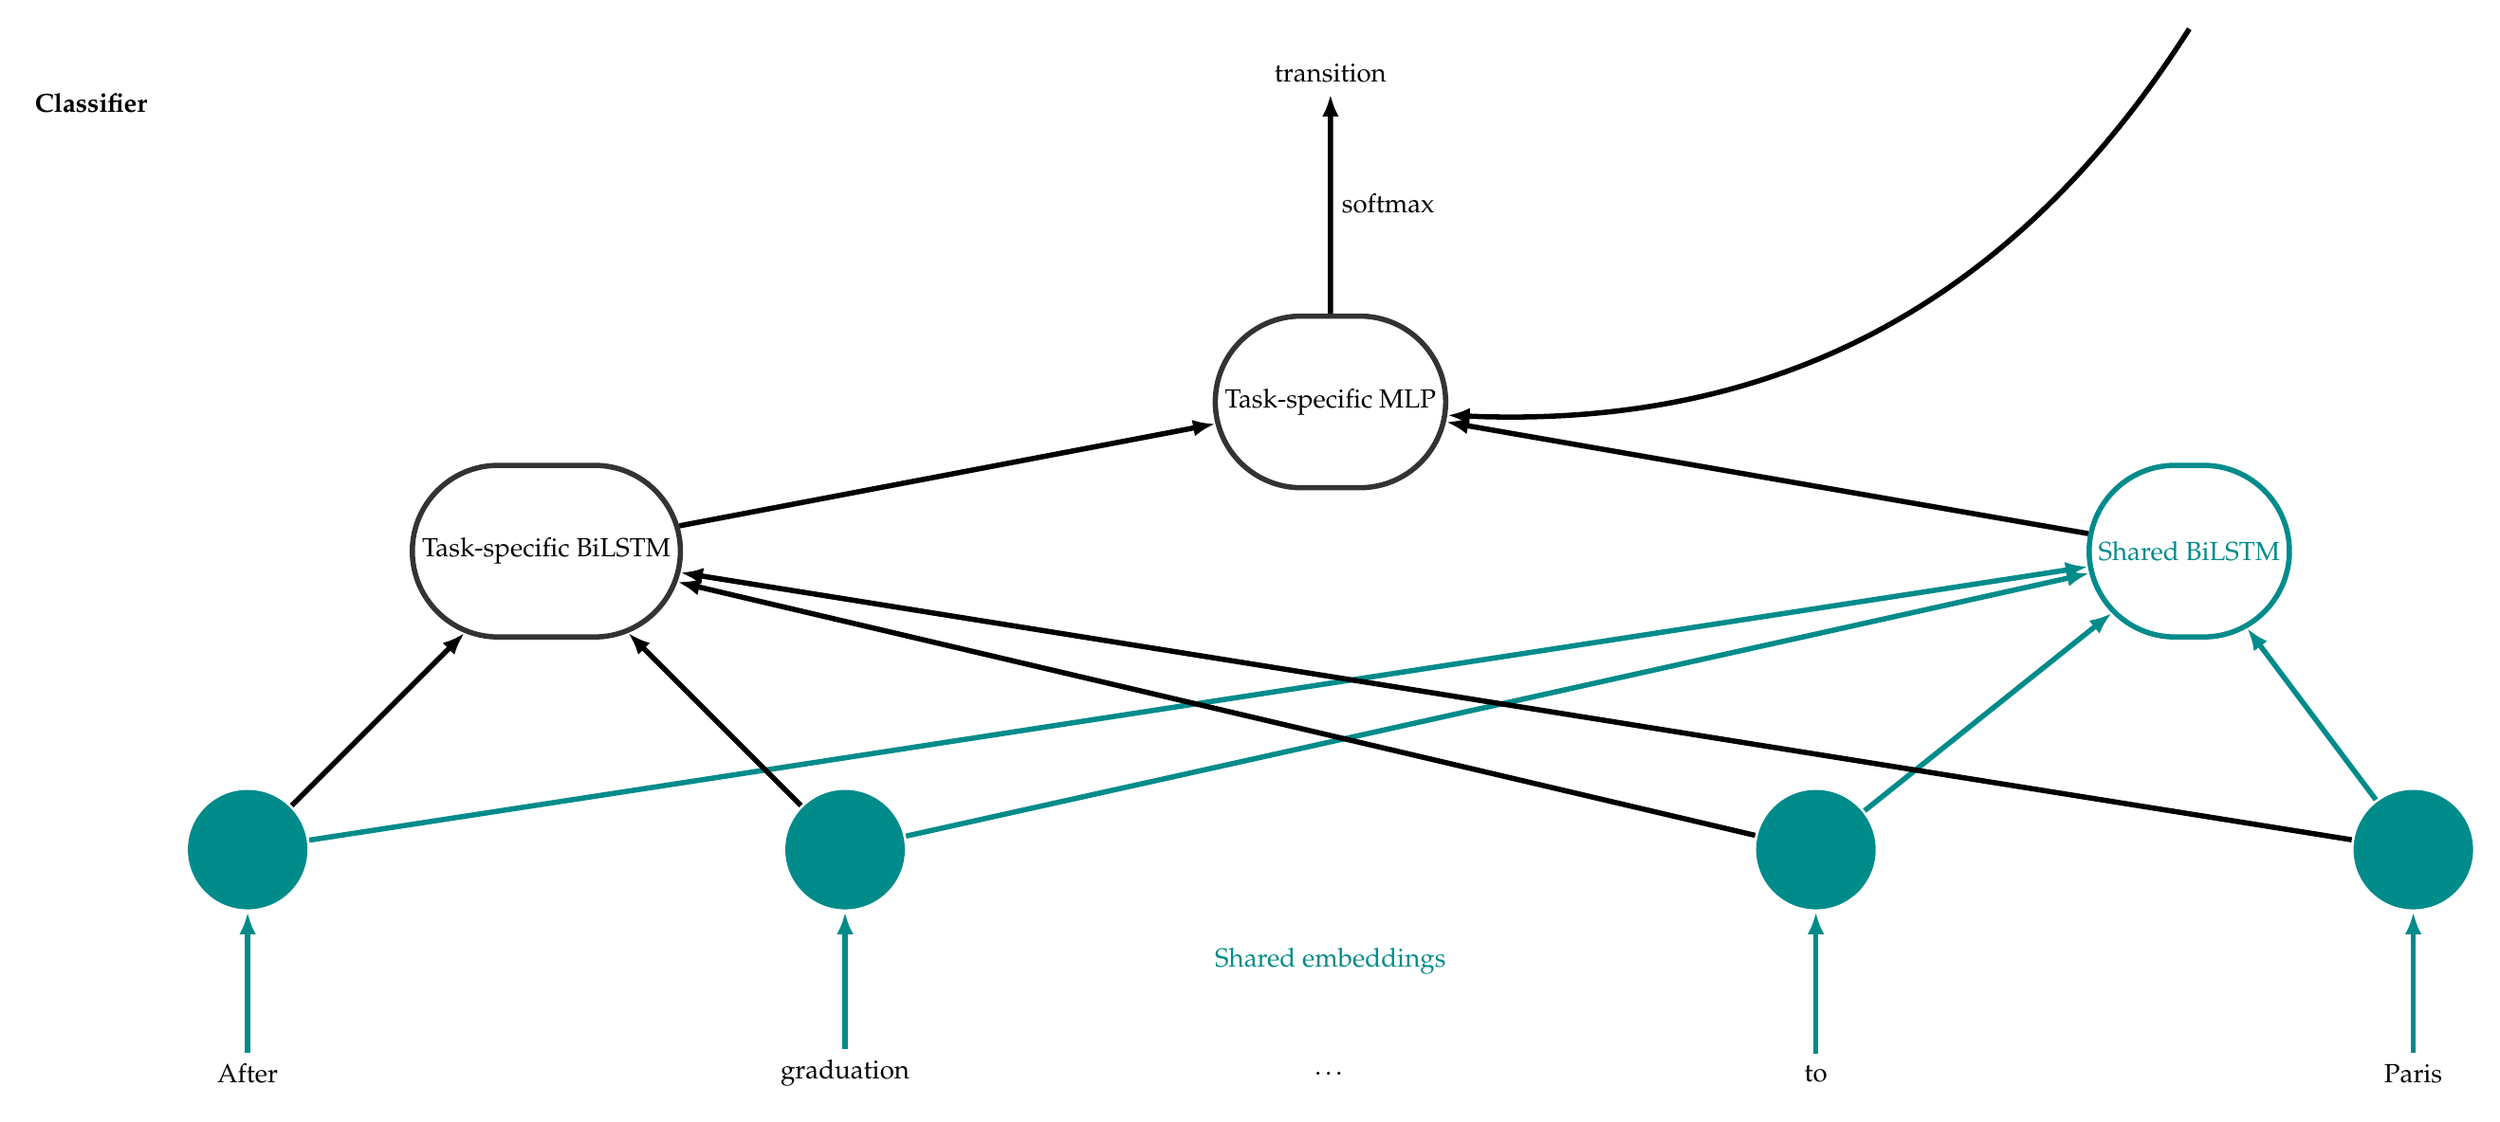
\begin{tikzpicture}[-{Latex[length=3mm]},thick, line width=2pt]
   \node[anchor=west] at (-7,16) {\textbf{Classifier}};
   \tikzstyle{main}=[rounded rectangle, minimum size=23mm, draw=black!80, node distance=12mm]
   \node[main] (specific) at (0,10) {Task-specific BiLSTM};
   \node[main,color=DarkCyan] (shared) at (22,10) {Shared BiLSTM};
   \node[color=DarkCyan] (embeddings) at (10.5,4.5) {Shared embeddings};
   \foreach \i/\word in {-4/{After},4/{graduation},17/{to},25/{Paris}} {
       \node (x\i) at (\i,3) {\word};
       \node[main, minimum size=16mm, fill=DarkCyan, draw=none] (e\i) at (\i,6) {};
       \path[color=DarkCyan] (x\i) edge (e\i);
       \path (e\i) edge (specific);
       \path[color=DarkCyan] (e\i) edge (shared);
   }
    \node (x4) at (10.5,3) {\ldots};
    \node[main] (mlp) at (10.5,12) {Task-specific MLP};
    \path (specific) edge (mlp);
    \path (shared) edge (mlp);
    \coordinate (state) at (22,17);
    \path (state) edge [bend left] (mlp);
    \node (transition) at (10.5,16.4) {transition};
    \path (mlp) edge node[right] {softmax} (transition);
   \end{tikzpicture}
\end{center}

Limited capacity promotes generalization by using the shared parameters for all tasks
\cite{E17-1005}.

\hrule

\section*{Unified DAG Format}

We convert all representations into a format similar to UCCA and
supported by TUPA.

\begin{minipage}{.4\columnwidth}
  \begin{center}
  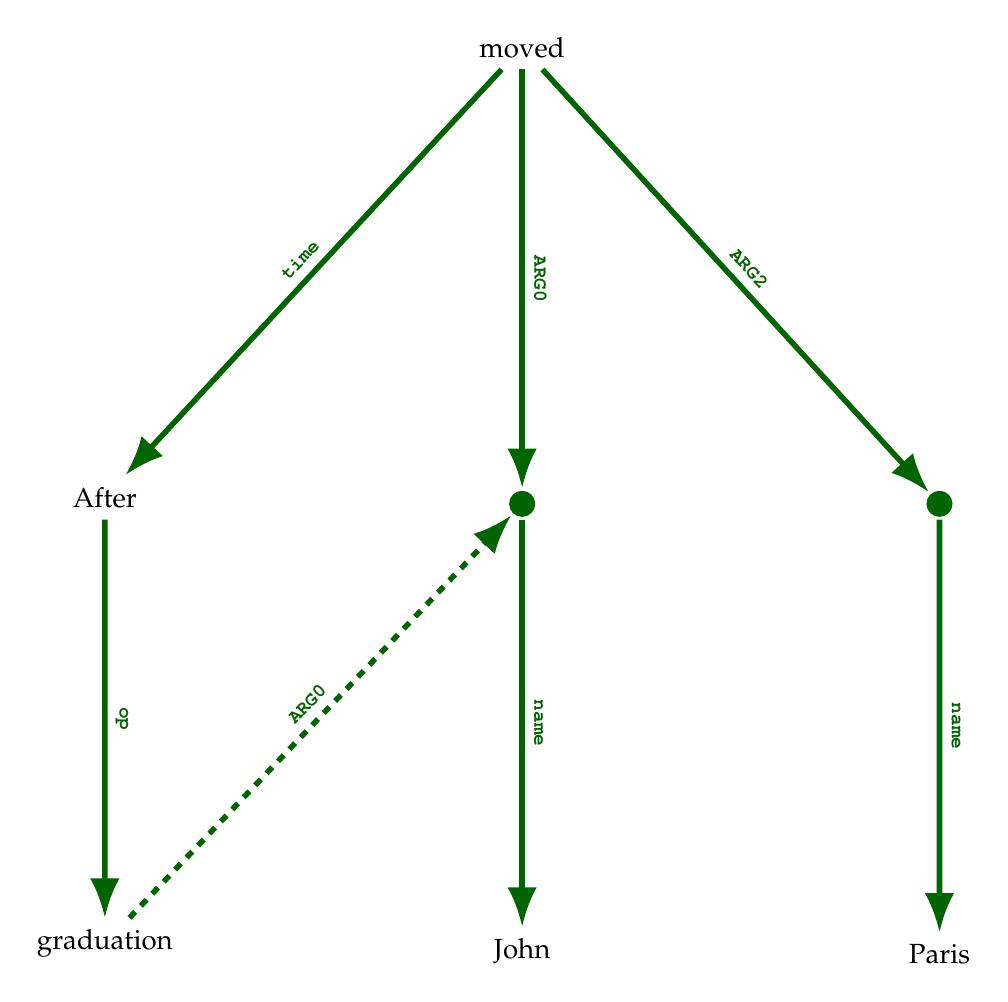
\begin{tikzpicture}[level distance=6cm, -{Latex[length=5mm]}, color=DarkGreen, line width=2pt,
      every node/.append style={sloped,anchor=south,auto=false,font=\scriptsize\bf\ttfamily},
      level 1/.style={sibling distance=53mm},
      level 2/.style={sibling distance=3cm},
      level 3/.style={sibling distance=3cm}]
    \tikzstyle{word} = [font=\rmfamily,color=black]
    \node (ROOT) [word] {moved}
      child {node [word] {After}
      {
            child {node (graduation) [word] {graduation} edge from parent node {op} }
      } edge from parent node {time} }
      child {node (John) [fill=DarkGreen,circle] {}
      {
        child {node [word] {John} edge from parent node {name} }
      } edge from parent node {ARG0} }
      child {node [fill=DarkGreen,circle] {}
      {
        child {node [word] {Paris} edge from parent node {name} }
      } edge from parent node {ARG2} }
      ;
      \draw[dashed] (graduation) to node {ARG0} (John);
  \end{tikzpicture}
  \captionof{figure}{\color{DarkGreen} Converted AMR.}
  \end{center}
\end{minipage}
\hfill
\begin{minipage}{.6\columnwidth}
  \begin{center}
  \scalebox{.9}{
  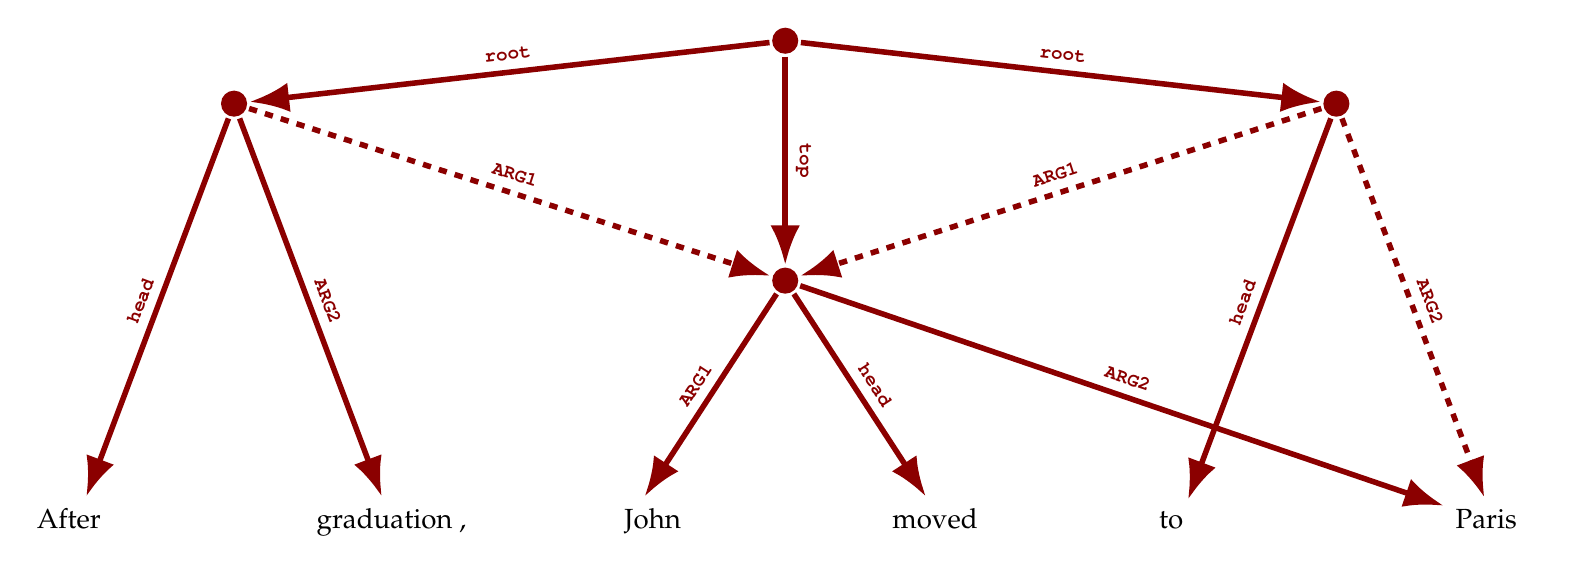
\begin{tikzpicture}[-{Latex[length=5mm]}, color=DarkRed, line width=2pt,
      every node/.append style={sloped,anchor=south,auto=false,font=\scriptsize\bf\ttfamily},
      level 1/.style={sibling distance=7cm,level distance=1cm},
      level 2/.style={sibling distance=4cm,level distance=24mm},
      level 3/.style={level distance=34mm}]
    \tikzstyle{word} = [font=\rmfamily,color=black]
    \node (ROOT) [fill=DarkRed,circle] {}
      child {node (after) [fill=DarkRed,circle] {}
      {
        child {node [draw=none] {}
        {
          child {node [word] (after_word) {After{\color{white}g}} edge from parent [draw=none]}
        } edge from parent [draw=none] }
        child {node [draw=none] {}
        {
          child {node [word] (graduation) {graduation ,} edge from parent [draw=none]}
        } edge from parent [draw=none] }
      } edge from parent node {root}}
      child {node [draw=none] {}
      {
        child {node (moved) [fill=DarkRed,circle] {}
        {
          child {node [word] {\quad{\color{white}g} John} edge from parent node {ARG1}}
          child {node [word] {moved{\color{white}g}} edge from parent node {head}}
        } edge from parent [draw=none] }
      } edge from parent [draw=none] }
      child {node (to) [fill=DarkRed,circle] {}
      {
        child {node [draw=none] {}
        {
            child {node [word] (to_word) {to{\color{white}g}} edge from parent [draw=none]}
          } edge from parent [draw=none] }
          child {node [draw=none] {}
        {
          child {node [word] (Paris) {Paris{\color{white}g}} edge from parent [draw=none]}
        } edge from parent [draw=none] }
      } edge from parent node {root}}
      ;
      \draw (ROOT) to node {top} (moved);
      \draw (after) to node {head} (after_word);
      \draw (after) to node {ARG2} (graduation);
      \draw[dashed] (after) to node {ARG1} (moved);
      \draw[dashed] (to) to node {ARG1} (moved);
      \draw (to) to node {head} (to_word);
      \draw (moved) to node {ARG2} (Paris);
      \draw[dashed] (to) to node {ARG2} (Paris);
  \end{tikzpicture}}
  \captionof{figure}{\color{DarkRed} Converted DM.}
  \scalebox{.9}{
  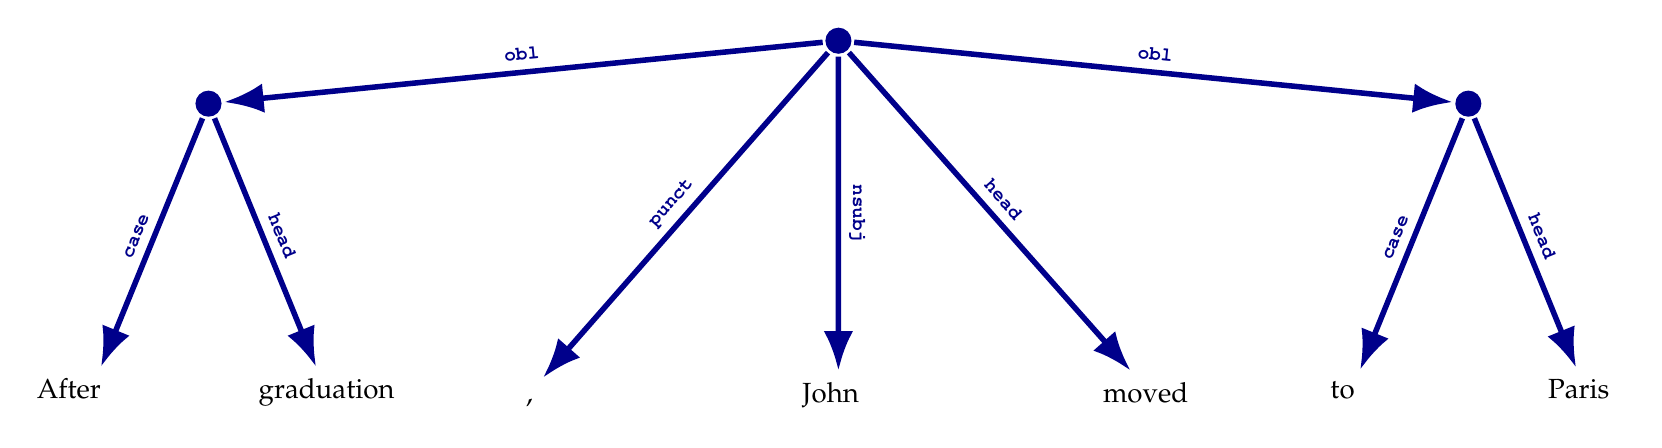
\begin{tikzpicture}[-{Latex[length=5mm]}, color=DarkBlue, line width=2pt,
      every node/.append style={sloped,anchor=south,auto=false,font=\scriptsize\bf\ttfamily},
      level 1/.style={sibling distance=4cm,level distance=1cm},
      level 2/.style={sibling distance=3cm,level distance=4cm}]
    \tikzstyle{word} = [font=\rmfamily,color=black]
    \node (ROOT) [fill=DarkBlue,circle] {}
      child {node (after) [fill=DarkBlue,circle] {}
      {
        child {node [word] {After{\color{white}g}\quad\quad} edge from parent node {case}}
        child {node [word] {\quad graduation\quad\quad} edge from parent node {head}}
      } edge from parent node {obl}}
      child {node {}
      {
        child {node [word] (comma) {\quad,{\color{white}g}} edge from parent [draw=none]}
      } edge from parent [draw=none]}
      child {node {}
      {
        child {node [word] (John) {John{\color{white}g}} edge from parent [draw=none]}
      } edge from parent [draw=none]}
      child {node {}
      {
        child {node [word] (moved) {moved{\color{white}g}} edge from parent [draw=none]}
      } edge from parent [draw=none]}
      child {node (to) [fill=DarkBlue,circle] {}
      {
          child {node [word] {to{\color{white}g}} edge from parent node {case}}
          child {node [word] {Paris{\color{white}g}} edge from parent node {head}}
      } edge from parent node {obl}}
      ;
      \draw (ROOT) to node {punct} (comma);
      \draw (ROOT) to node {nsubj} (John);
      \draw (ROOT) to node {head} (moved);
  \end{tikzpicture}}
  \captionof{figure}{\color{DarkBlue} Converted UD.}
  \end{center}
\end{minipage}

\hrule



\section*{Experiments}

\textbf{English}. Train: {\color{Indigo} UCCA Wiki}
(+aux), test: {\color{Indigo} UCCA Wiki} (in-domain) or
{\color{Indigo} 20K} (out-of-domain).
\textbf{French} and \textbf{German}. Train: {\color{Indigo} 20K}
(+{\color{DarkBlue} UD} as aux),
test: {\color{Indigo} 20K} (both in-domain).
\pgfplotstableread[row sep=\\,col sep=&]{
	aux & pf1 & rf1 \\
	+All & 74.4 & 52 \\
	+{\color{DarkRed} \textbf{SDP}} + {\color{NavyBlue} \textbf{UD}} & 74.9 & 51.2 \\
	+{\color{DarkGreen} \textbf{AMR}} + {\color{NavyBlue} \textbf{UD}} & 73.8 & 48.5 \\
	+{\color{DarkGreen} \textbf{AMR}} + {\color{DarkRed} \textbf{SDP}} & 74.7 & 51.4 \\
	+\color{NavyBlue} \textbf{UD} & 74.1 & 50.8 \\
	+\color{DarkRed} \textbf{SDP} & 74.8 & 53.9 \\
	+\color{DarkGreen} \textbf{AMR} & 73.7 & 49.9 \\
	\textbf{Single-task} & 73.6 & 51.5 \\
}\indomaindata

\pgfplotstableread[row sep=\\,col sep=&]{
	aux & pf1 & rf1 \\
	+All & 71 & 29.6 \\
	+{\color{DarkRed} \textbf{SDP}} + {\color{NavyBlue} \textbf{UD}} & 70.6 & 28.4 \\
	+{\color{DarkGreen} \textbf{AMR}} + {\color{NavyBlue} \textbf{UD}} & 70 & 29.4 \\
	+{\color{DarkGreen} \textbf{AMR}} + {\color{DarkRed} \textbf{SDP}} & 70.5 & 27.3 \\
	+\color{NavyBlue} \textbf{UD} & 69.7 & 28.7 \\
	+\color{DarkRed} \textbf{SDP} & 70.7 & 25.9 \\
	+\color{DarkGreen} \textbf{AMR} & 69.5 & 27.5 \\
	\textbf{Single-task} & 69 & 26.7 \\
}\outdomaindata

\pgfplotstableread[row sep=\\,col sep=&]{
	aux & pf1 & rf1 \\
	+\color{NavyBlue} \textbf{UD} & 70.1 & 20.3 \\
	\textbf{Single} & 67.6 & 13.9 \\
}\frenchdata

\pgfplotstableread[row sep=\\,col sep=&]{
	aux & pf1 & rf1 \\
	+\color{NavyBlue} \textbf{UD} & 73.2 & 35.5 \\
	\textbf{Single} & 72.5 & 27.1 \\
}\germandata

\begin{center}
    \small
	\begin{minipage}{.45\columnwidth}
	\begin{tikzpicture}
		    \begin{axis}[
		    xbar,
		    width=11cm,
		    height=18cm,
		    xmin=47,
		    xmax=80,
		    bar width=7mm,
		    xtick=\empty,
		    ytick=data,
		    yticklabels from table={\indomaindata}{aux},
		    axis x line=none,
		    axis line style={draw=none},
		    clip=false
		    ]
		    \addplot [fill=Crimson, point meta=explicit symbolic,nodes near coords,
		    nodes near coords align={anchor=west}] table [x=rf1,y expr=\coordindex,meta=rf1] {\indomaindata};
		    \addplot [fill=Navy, point meta=explicit symbolic,nodes near coords,
		    nodes near coords align={anchor=west}] table [x=pf1,y expr=\coordindex,meta=pf1] {\indomaindata};
		    \end{axis}
	\end{tikzpicture}
	\captionof{figure}{English In-Domain.}
	\end{minipage}
	\begin{minipage}{.30\columnwidth}
	\begin{tikzpicture}
		    \begin{axis}[
		    xbar,
		    width=11cm,
		    height=18cm,
		    xmin=23,
		    xmax=77,
		    bar width=7mm,
		    xtick=\empty,
		    axis x line=none,
		    axis y line=none,
		    clip=false
		    ]
		    \addplot [fill=Crimson, point meta=explicit symbolic,nodes near coords,
		    nodes near coords align={anchor=west}] table [x=rf1,y expr=\coordindex,meta=rf1] {\outdomaindata};
		    \addplot [fill=Navy, point meta=explicit symbolic,nodes near coords,
		    nodes near coords align={anchor=west}] table [x=pf1,y expr=\coordindex,meta=pf1] {\outdomaindata};
		    \end{axis}
	\end{tikzpicture}
	\captionof{figure}{English Out-of-Domain.}
	\end{minipage}
	\begin{minipage}{.21\columnwidth}
	\begin{tikzpicture}
		    \begin{axis}[
		    xbar,
		    width=7cm,
		    height=5cm,
		    xmin=10,
		    xmax=80,
		    bar width=7mm,
		    xtick=\empty,
		    ytick=data,
		    yticklabels from table={\frenchdata}{aux},
		    axis x line=none,
		    axis line style={draw=none},
		    clip=false
		    ]
		    \addplot [fill=Crimson, point meta=explicit symbolic,nodes near coords,
		    nodes near coords align={anchor=west}] table [x=rf1,y expr=\coordindex,meta=rf1] {\frenchdata};
		    \addplot [fill=Navy, point meta=explicit symbolic,nodes near coords,
		    nodes near coords align={anchor=west}] table [x=pf1,y expr=\coordindex,meta=pf1] {\frenchdata};
		    \end{axis}
	\end{tikzpicture}
	\captionof{figure}{French (in-domain).}

    \vspace{5mm}
	
	\begin{tikzpicture}
		    \begin{axis}[
		    xbar,
		    width=7cm,
		    height=5cm,
		    xmin=10,
		    xmax=80,
		    bar width=7mm,
		    reverse legend,
	        legend style={at={(axis cs:0,1.5)},anchor=south west},
		    xtick=\empty,
		    ytick=data,
		    yticklabels from table={\germandata}{aux},
		    axis x line=none,
		    axis line style={draw=none},
		    clip=false
		    ]
		    \addplot [fill=Crimson, point meta=explicit symbolic,nodes near coords,
		    nodes near coords align={anchor=west}] table [x=rf1,y expr=\coordindex,meta=rf1] {\germandata};
		    \addplot [fill=Navy, point meta=explicit symbolic,nodes near coords,
		    nodes near coords align={anchor=west}] table [x=pf1,y expr=\coordindex,meta=pf1] {\germandata};
		    \legend{remote F1,primary F1}
		    \end{axis}
	\end{tikzpicture}
	\captionof{figure}{German (in-domain).}
	\end{minipage}
\end{center}

Multitask learning consistently improve UCCA parsing when compared to single-task.

\hrule


\section*{Task Similarity}

\pgfplotstableread[row sep=\\,col sep=&]{
	aux & cpf1 & crf1 & l1 \\
	\color{NavyBlue} \textbf{UD} & 83.6 & 12.6 & 84.3 \\
	\color{DarkRed} \textbf{SDP} & 56 & 13.3 & 91.3 \\
	\color{DarkGreen} \textbf{AMR} & 24.2 & 6.3 & 89.5 \\
}\similaritydata

Does improvement depend on structural task similarity,
or training corpus similarity? \\
We compared
\textbf{\color{NavyBlue} annotations of 100 WSJ sentences},
and \textbf{\color{DarkGreen} training corpus word distributions}.

\begin{tikzpicture}
	    \begin{axis}[
	    xbar,
	    width=22cm,
	    height=8cm,
	    xmin=0,
	    xmax=105,
		bar width=7mm,
	    xtick=\empty,
	    ytick=data,
	    yticklabels from table={\similaritydata}{aux},
	    reverse legend,
        legend style={at={(axis cs:105,1)},anchor=west,cells={align=left},row sep=6mm,font=\small},
	    axis x line=none,
		axis line style={draw=none},
	    clip=false
	    ]
	    \addplot [fill=Green, point meta=explicit symbolic,nodes near coords,
	    nodes near coords align={anchor=west}] table [x=l1,y expr=\coordindex,meta=l1] {\similaritydata};
	    \addplot [fill=Red, point meta=explicit symbolic,nodes near coords,
	    nodes near coords align={anchor=west}] table [x=crf1,y expr=\coordindex,meta=crf1] {\similaritydata};
	    \addplot [fill=Blue, point meta=explicit symbolic,nodes near coords,
	    nodes near coords align={anchor=west}] table [x=cpf1,y expr=\coordindex,meta=cpf1] {\similaritydata};
	    \legend{,unigram distribution L1 distance \\ ($\times 100$; compared to UCCA Wiki),
	             unlabeled remote F1 \\ (compared to gold UCCA on WSJ),
	             unlabeled primary F1 \\ (compared to gold UCCA on WSJ)}
	    \end{axis}
\end{tikzpicture}


\begin{multicols}{2}
\color{DarkSlateGray}
\tiny\titleformat*{\section}{\small}
\bibliographystyle{plain}
\bibliography{references}

\color{Black}
\begin{adjustbox}{margin=3mm,frame,minipage=\columnwidth}
\centering\large
Please join SemEval 2019 Task 1: \\
Cross-lingual Semantic Parsing with UCCA

\begin{minipage}{.3\textwidth}
\includegraphics[width=\textwidth]{qr}\end{minipage}
\hfill
\begin{minipage}{.6\textwidth}\Large\url{tinyurl.com/semeval-ucca}\end{minipage}
\end{adjustbox}
\end{multicols}

\end{multicols}
\end{document}
